\section{Theory}
\label{sec:Theory}

\subsection{X-ray radiation}
X-ray radiation is a type of electromagnetic radiation with a wavelength of $\qty{10}{\nano\meter}$ to $\qty{10}{\pico\meter}$.
In this experiment the radiation is obtained by an x-ray tube.
\begin{figure}
    \centering
    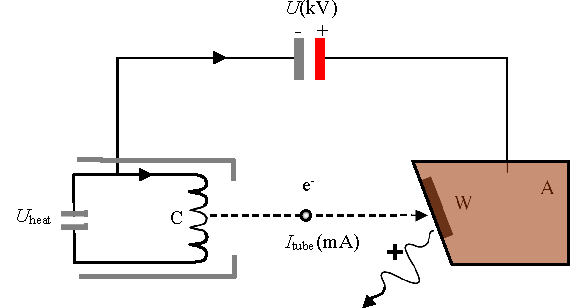
\includegraphics[width=0.6\textwidth]{images/x-ray_tube.pdf}
    \caption{Schematic representation of an x-ray tube. \cite{V44:strahlung_krieger}}
    \label{fig:x-ray_tube}
\end{figure}
The process of generating x-ray radiation in an x-ray tube is shown in \autoref{fig:x-ray_tube}.
In an x-ray tube electrons are emitted by an incandescent wire inside the tube.
They are accelerated by a high voltage between the cathode $C$ and the anode $A$, in this case copper.
When the electron hits the anode it interacts with the coulomb fields of the atoms in the anode.
During this interaction the electron emits bremsstahlung and ionizes the atoms, it can't interact with other atoms before because of the vacuum in the tube.
This results in two different kinds of radiation: the continuous bremsstrahlung and the discrete x-ray radiation.
In this experiment mainly the characteristic radiation is used.

\subsection{Reflection at one interface}
X-ray radiation behaves differently if reflecting at one interface or multiple interfaces.
If the radiation hits one flat surface the refractive index $n$ is described by
\begin{equation}
    n = 1 - \delta + \symup{i}\beta,
    \label{eqn:ndelta}
\end{equation}
with the dispersive component $\delta\,\left[\mathcal{O}\left(10^{-6}\right)\right]$and the absorptive component $\beta\,\left[\mathcal{O}\left(10^{-7}\right)\right]$.
Equation \eqref{eqn:ndelta} shows that the refractive index for x-ray radiation is always $n < 1$.
\begin{figure}
    \centering
    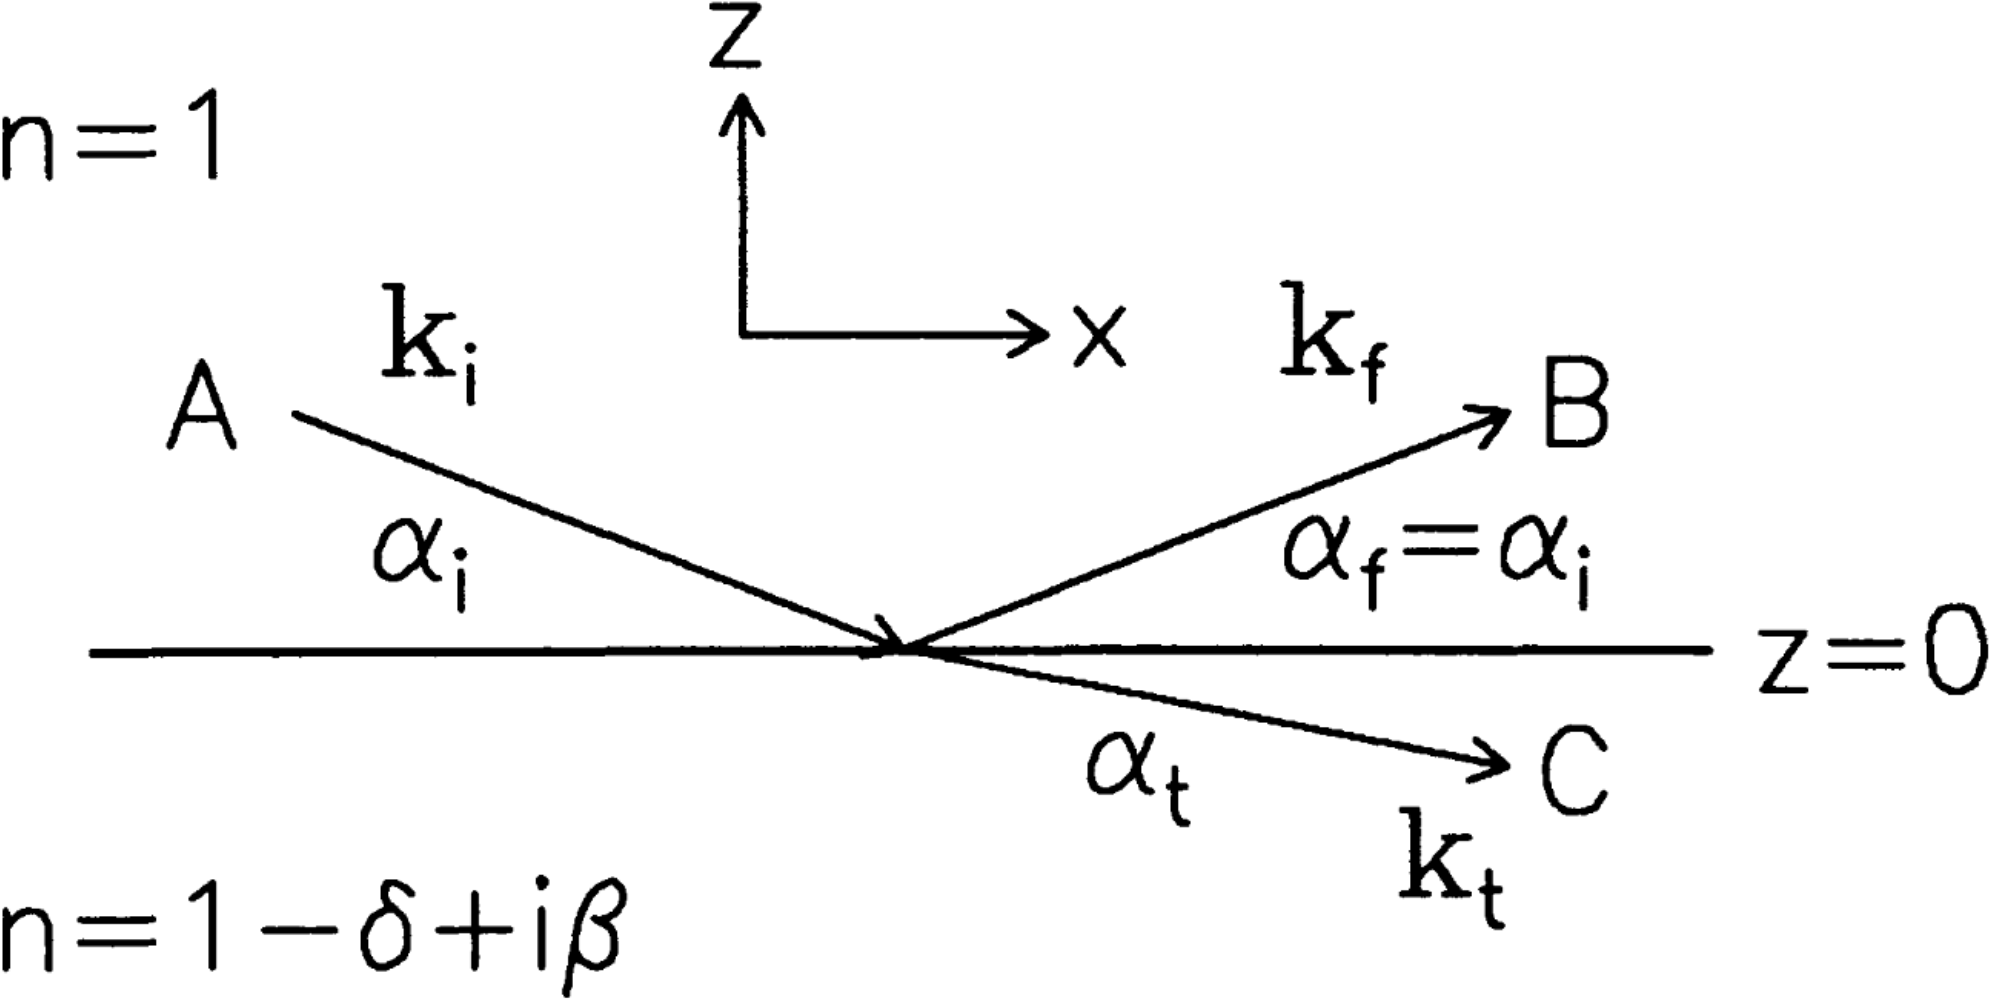
\includegraphics[width=0.6\textwidth]{images/scattering.png}
    \caption{Schematic representation of the reflection and transmission of x-ray radiation.
    Due to $n<1$ the transmitted part is refracted away from the optical normal \cite[7]{V44:xrr_tolan}.}
    \label{fig:reflection}
\end{figure}
This results in the possibility of total reflection in a vacuum below a certain angle $\alpha_\text{c}$.
This can be used with Snell's Law
\begin{equation*}
    \frac{n_1}{n_2} = \frac{\cos\l(\alpha_1\r)}{\cos\l(\alpha_2\r)}
\end{equation*}
and under the assumption of $\beta\approx0$ to calculate the critical angle with 
\begin{equation}
    \alpha_\text{c} = \sqrt{2\delta} = \lambda\sqrt{\frac{r_\text{e}\cdot\rho}{\symup{\pi}}}.
    \label{eqn:critical_angle}
\end{equation}

\subsection{Fresnel equations}
The interaction of electromagnetic radiation with an optical medium can be described by the Fresnel equations.
Depending on the polarization of the light, different equations need to be used.
In this case the refractive indices $n_1\approx n_2$ are very similar \cite[8]{V44:xrr_tolan} therefore the equations become the same
\begin{align}\label{eqn:fresnel}
    r &= \frac{n_1\cos\l(\alpha_1\r)-n_2\cos\l(\alpha_2\r)}{n_1\cos\l(\alpha_1\r)+n_2\cos\l(\alpha_2\r)} \\
    t &= \frac{2n_1}{n_1\cos\l(\alpha_1\r)+n_2\cos\l(\alpha_2\r)}.
\end{align}
$r$ is the amplitude of the reflected and $t$ of the transmitted light.
$n_1$ and $n_2$ are the refractive indices of the two media and $\alpha_1$ and $\alpha_2$ the angles of the reflected and transmitted light.
If the incident angle is more than three times larger than the critical angle $\alpha_\text{i} > 3\alpha_\text{c}$ \cite[9]{V44:xrr_tolan}, the Fresnel reflectivity can be calculated with
\begin{equation*}
    R_\text{F} \simeq \left(\frac{\alpha_\text{c}}{2\alpha_\text{i}}\right)^4.
    \label{eqn:fresnel_rflectivity}
\end{equation*}
\newpage

\subsection{Refraction at multiple interfaces}
If x-ray radiation hits a multi-layer system, the light gets reflected and transmitted at every single layer.
This is shown in \autoref{fig:multi_layer}.
\begin{figure}
    \centering
    \hfill
    \begin{subfigure}{0.47\textwidth}
        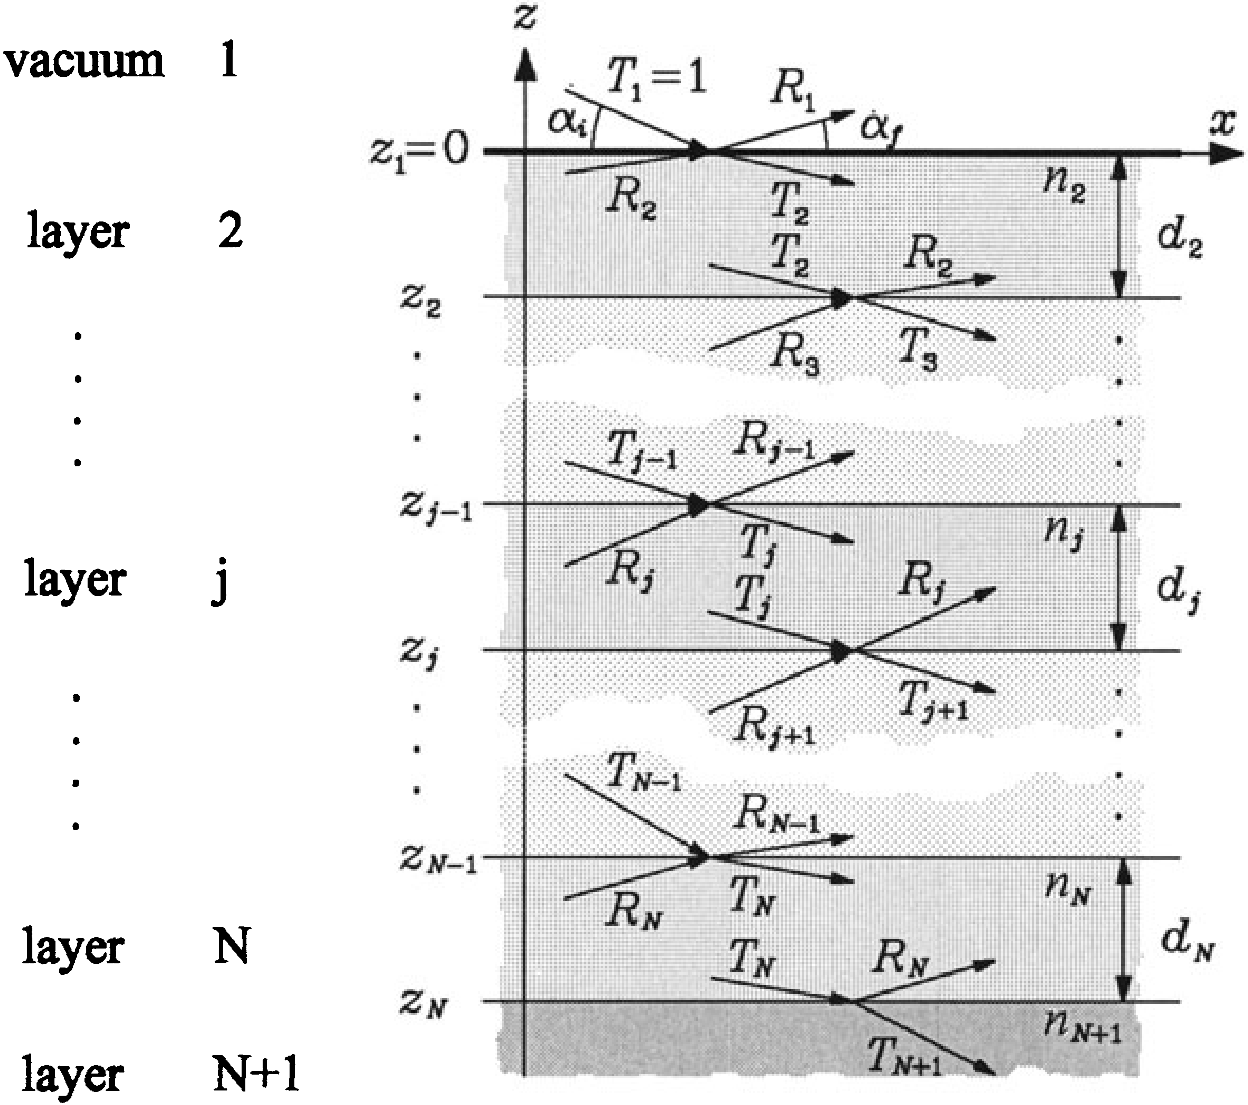
\includegraphics[width=\textwidth]{images/multi_layer.png}
        \caption{Interaction of x-ray radiation with a multi-layer system.
        The radiation gets transmitted and reflected at every layer.\\}
        \label{fig:multi_layer}
    \end{subfigure}
    \hfill
    \begin{subfigure}{0.47\textwidth}
        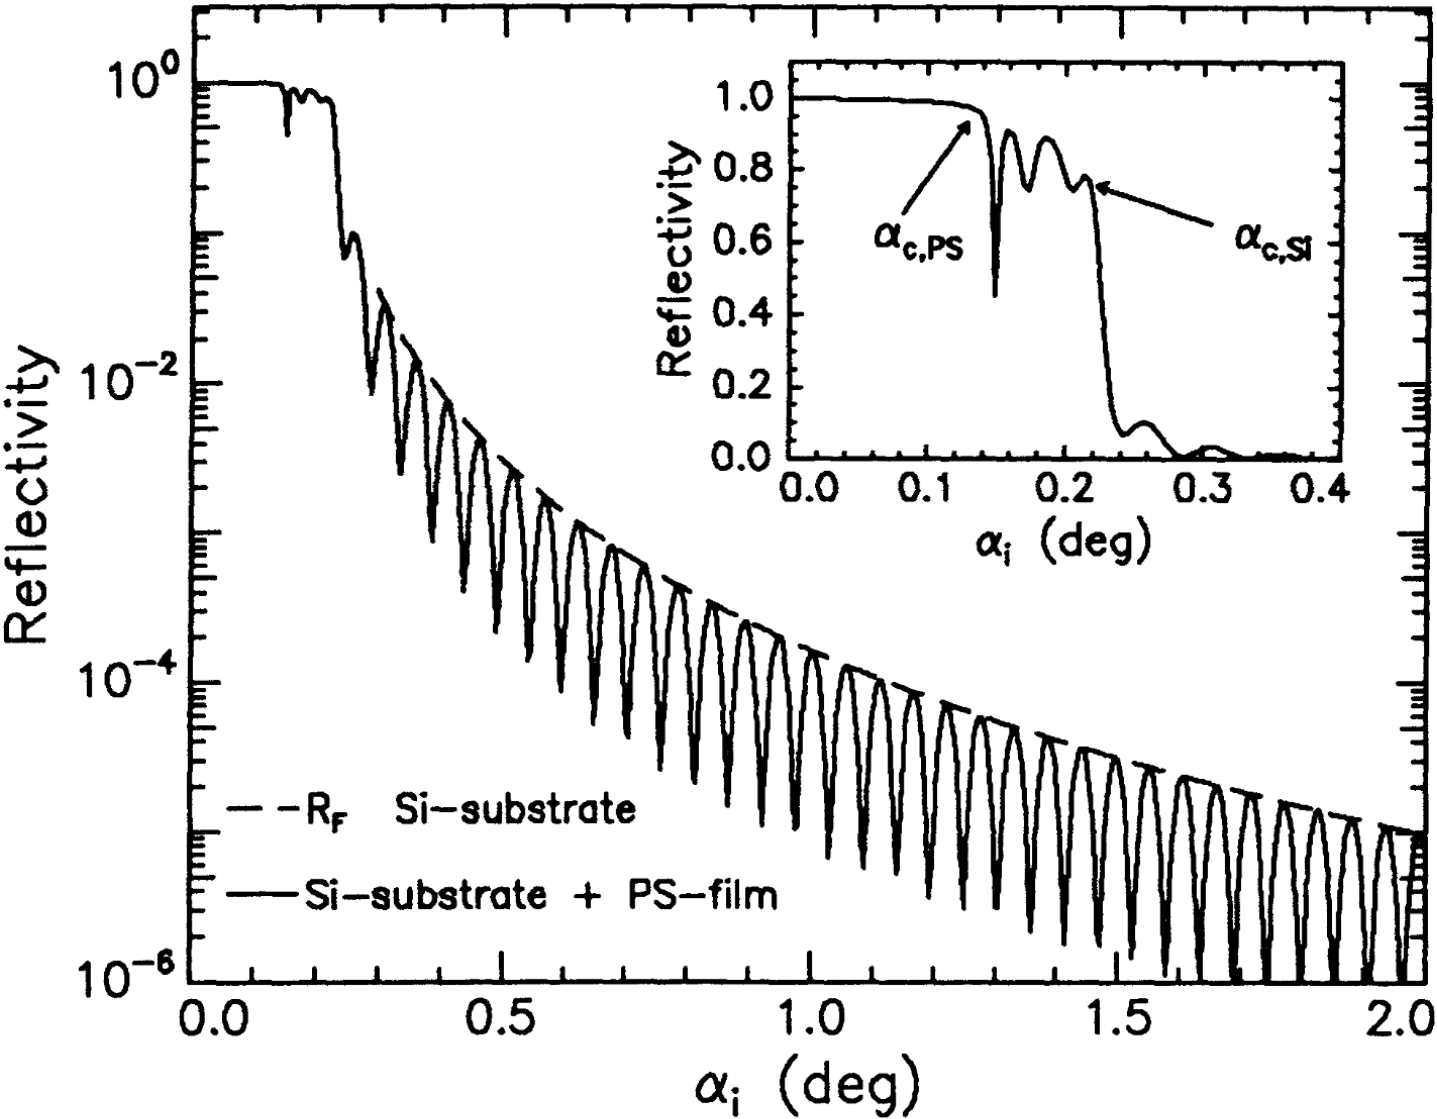
\includegraphics[width=\textwidth]{images/kiessig_oszillation.png}
        \caption{Reflectivity curve of a two layer system.
        The Kiessig oscillations are shown here.
        In the upper right the critical angles of polysterene and silicic are shown.}
        \label{fig:kiessig}
    \end{subfigure}
    \caption{Schematic representation of the reflection and transmission of x-ray radiation in a multilayer system and the resulting Kiessig oscillations \cite[12--14]{V44:xrr_tolan}.}
    \label{fig:ml_kiessig}
    \hfill
\end{figure}
The transmitted radiation can pass through the upper layer and interfere with the other reflected parts of the other layers.
Through the interference the intensity of the reflection begins to oscillate, as shown in \autoref{fig:kiessig}.
These oscillations are called Kiessig oscillations.
The layer thickness can be calculated through these oscillations with
\begin{equation}
    d = \frac{2\symup{\pi}}{\increment q_z} \approx \lambda \frac{1}{2\increment\alpha_\text{i}}.
    \label{eqn:thickness}
\end{equation}
$q_z$ is the $z$-component of the wave vector transfer $q=\vec{k_\text{f}}-\vec{k_\text{i}}$ (shown in \autoref{fig:reflection}) and can be obtained with $q_z=2k\sin\l(\alpha_\text{i}\r)$ \cite[14]{V44:xrr_tolan}.
The oscillations can be calculated with the recursive Parratt algorithm.
Its main idea is to approximate the lowest layer as a layer with infinite thickness.
On the lowest layer there will be no reflected part form below.
This results in the starting condition of $R_{N+1}=X_{N+1}=0$ for Equation \eqref{eqn:parratt}.
From that layer the reflectivity can be calculated for every layer on top of the previous.
This results in the recursive formula \cite[12]{V44:xrr_tolan}\cite{V44:parratt}
\begin{equation}
    X_j = \frac{R_j}{T_j} = \frac{r_{j,j+1}\,+\,X_{j+1}\,\exp\l(2\i\,k_{z,j+1}z_j\r)}{1+r_{j,j+1}X_{j+1}\exp\l(2\i\,k_{z,j+1}z_j\r)}.
    \label{eqn:parratt}
\end{equation}
$r_{j,j+1}$ can be calculated with $r_{j,j+1}=\frac{k_{z,j}-k_{z,j+1}}{k_{z,j}+k_{z,j+1}}$ and represents the Fresnel coefficient of the $j$-th layer.

\subsubsection{Rough interfaces}
The formula \eqref{eqn:parratt} only holds for plain surfaces.
In reality all surfaces are rough.
To use the Parratt algorithm this has to be taken into account.
\begin{figure}
    \centering
    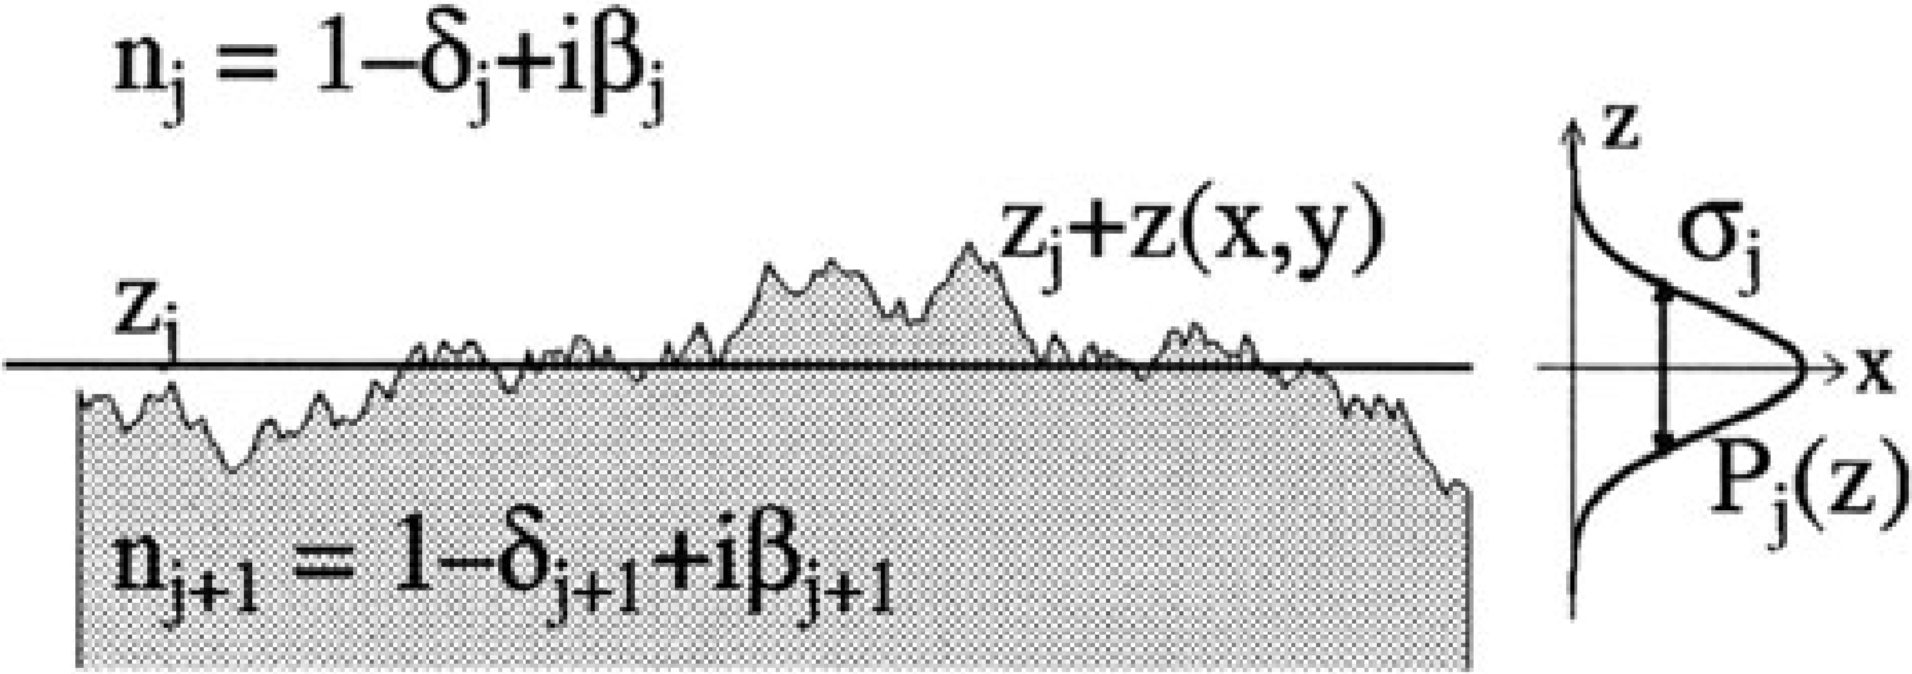
\includegraphics[width=0.5\textwidth]{images/rough.png}
    \caption{Schematic representation of a rough interface.
    The roughness gets approximated by different plain surfaces at height $z_j+z$ through the probability distribution $P_j$ \cite[15]{V44:xrr_tolan}.}
    \label{fig:rough}
\end{figure}
The rough surface gets approximated by an ensemble of even surfaces (shown in \autoref{fig:rough}) which are calculated by the root-mean-square roughness
\begin{equation*}
    \sigma^2 = \int \l(z-\mu_j\r) P_j\l(z\r) \diff{z} = \int \l(z-z_j\r) P_j\l(z\r) \diff{z}. \\
\end{equation*}
$P_j$ is the probability distribution of the particular surface, in this case the Gaussian distribution, and $\mu_j$ is the mean value, in this case $z_j$.
This results in the modified Fresnel formula
\begin{equation}
    \tilde{r}_{j+1,j} = r_{j,j+1}\exp\l(-2k_{z,j}k_{z,j+1}\sigma^2\r),
\end{equation}
without the $\tilde{t}$ as it cancels itself in the Parratt algorithm.
This modified Parratt algorithm can only be used if the roughness is much smaller than the thickness of the layers e.g., $\sigma_j\ll d_j$.

\begin{figure}
    \hfill
    \begin{subfigure}{0.35\textwidth}
        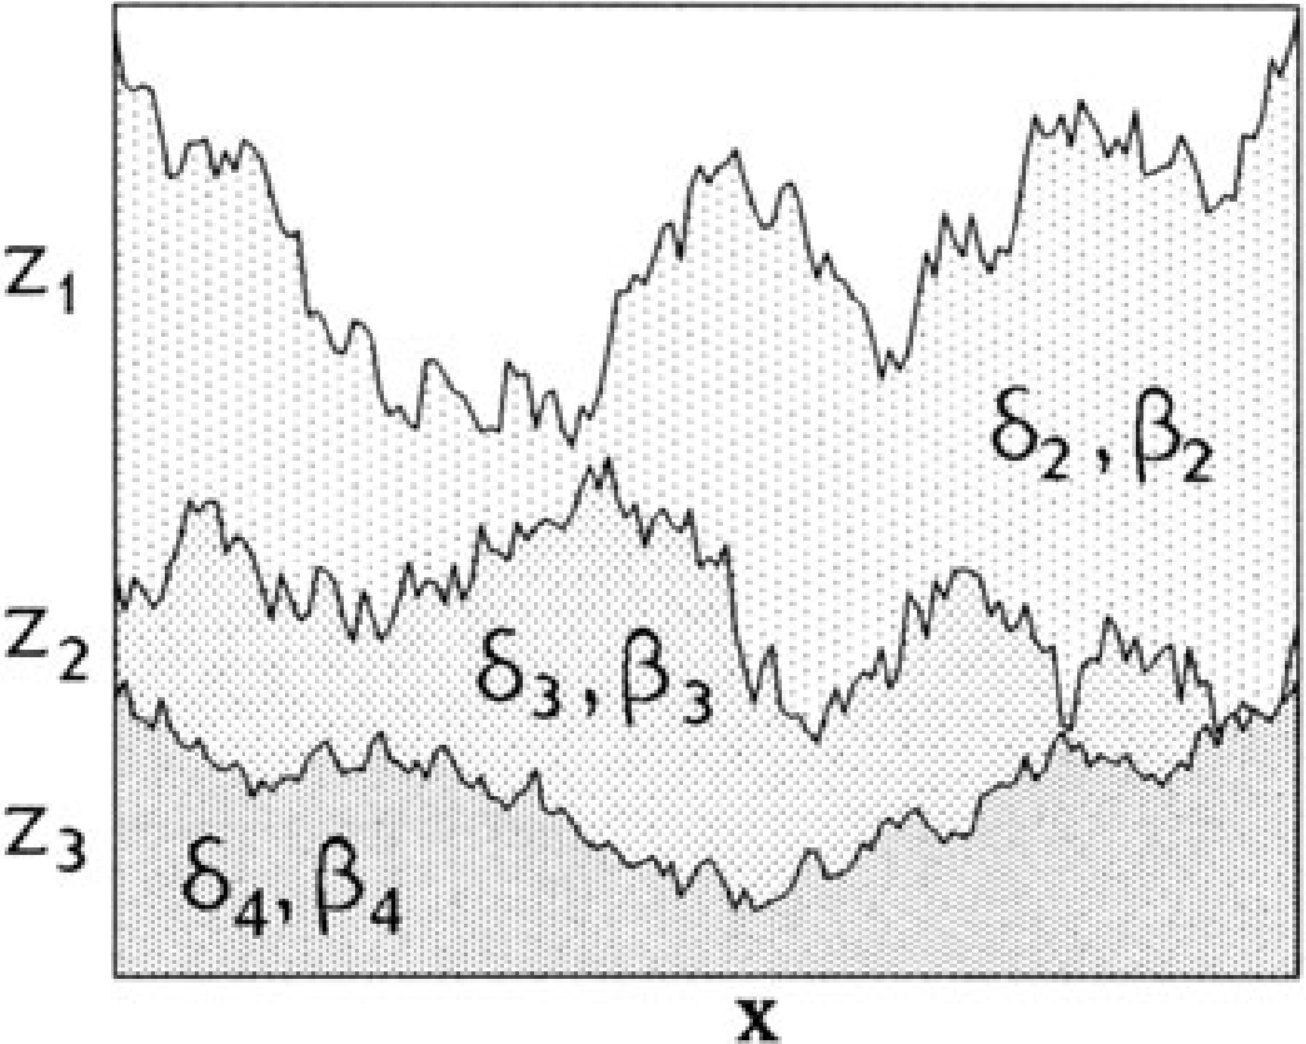
\includegraphics[width=\textwidth]{images/rough_layer.png}
        \caption{Schematic representation of a very rough multi-layer system.}
    \end{subfigure}
    \hfill
    \begin{subfigure}{0.35\textwidth}
        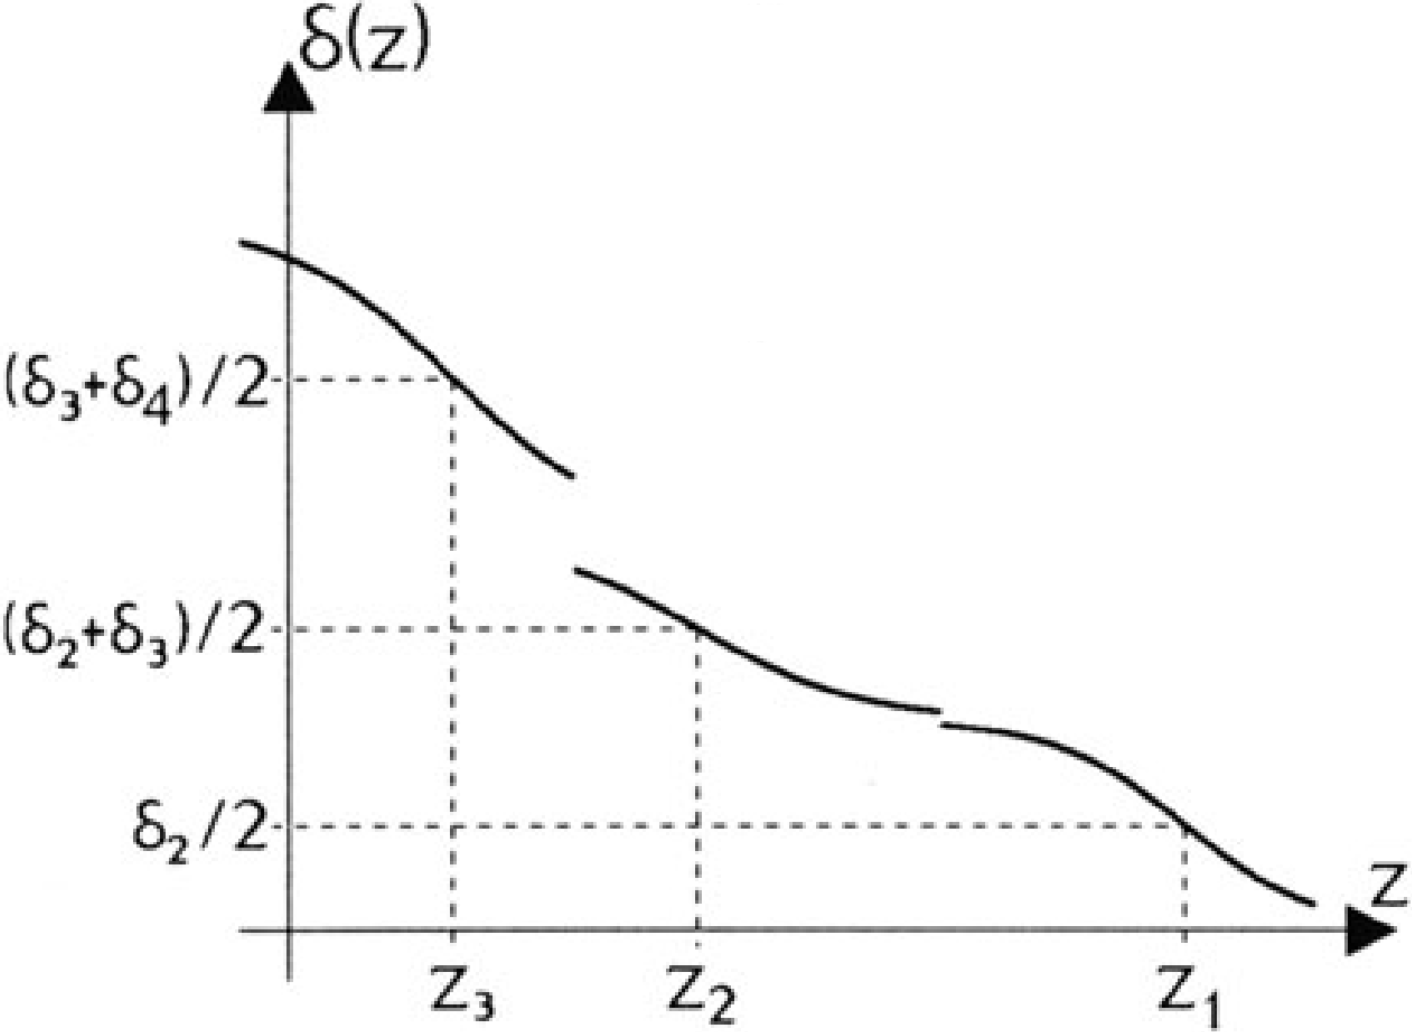
\includegraphics[width=\textwidth]{images/rough_function.png}
        \caption{Profile function of the very rough multi-layer system.}
    \end{subfigure}
    \caption{Schematic representation of a very rough multi-layer system with its profile function \cite[28]{V44:xrr_tolan}.}
    \label{fig:independent_layers}
    \hfill
\end{figure}

For systems with greater roughness it is necessary to model the roughnesses through independent layers with varying refractive indices and roughness.
The new profile isn't continuous and has to be modified iteratively to model the real surface as close as possible.
In \autoref{fig:independent_layers} is an example with a very rough surface and the resulting dispersion profile \cite[28]{V44:xrr_tolan}.

\subsection{Geometry factor}
In this experiment the x-ray beam will be reflected under different angles.
Due to the extent of the beam, the beam covers more area than the sample under small angles, as shown in \autoref{fig:beam_width}.
\begin{figure}
    \centering
    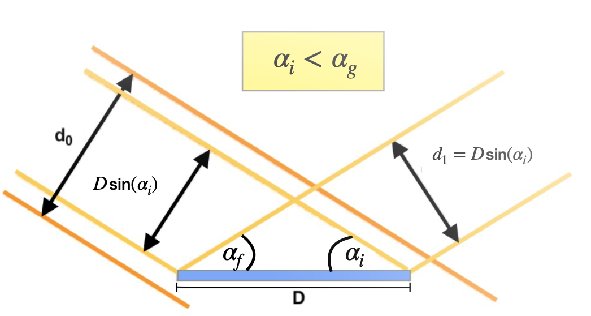
\includegraphics[width=0.6\textwidth]{images/beam_width.pdf}
    \caption{Schematic representation of the covered surface by the beam under small angles \cite{V44}.}
    \label{fig:beam_width}
\end{figure}
For all angles $\alpha < \arcsin\l(\frac{b_\text{i}}{l}\r)$, with the length $l$ of the sample and the beam width $b_\text{i}$, the surface covered by the beam is larger than the surface of the sample itself \cite[41--42]{V44:xrr_tolan}\cite{V44:parratt}.
This can be corrected with the geometry factor
\begin{equation}\label{eqn:geometry_factor}
    G =
    \begin{cases}
        \frac{D\sin\l(\alpha_\text{i}\r)}{d_0}, &\alpha_\text{i}<\alpha_\text{g}\\
        1, &\alpha_\text{i}>\alpha_\text{g},
    \end{cases}
\end{equation}
with the total beam width $d_0$ and the effective beam area $D\sin\l(\alpha_\text{i}\r)$ \cite{V44}.